%!TEX encoding = UTF-8 Unicode

%!TEX root = ../compendium.tex


\Lab{\LabWeekFOUR}

\begin{Goals}
\item Kunna använda utvecklingsmiljön Eclipse och dess ScalaIDE.
\item Kunna använda case classer för att spara data.
\item Kunna spara data till fil.
\item Kunna l{\"a}sa in data fr{\aa}n fil med \code{scala.io}.
\item Kunna skapa och använda klasser för att behandla data.
\item Kunna använda samlingstyperna vektor och map.
\item Förstå skillnaden mellan kompileringsfel och exekveringsfel.
\item Kunna felsöka (små) program med hjälp av utskrifter och debuggern i Eclipse.

%\item Att spara objekt till fil.
%\item Att l{\"a}sa in objekt fr{\aa}n en fil.
\end{Goals}

\begin{Preparations}
\item G{\"o}r {\"o}vning 4. % ref
\item Läs om Eclipse i Appendix.
\item Läs igenom laborationen och gör förberedelseuppgiften.
%\item {\"O}ppna Scala IDE i Eclipse enligt intruktionerna XX.
%\item Skapa ett projekt och skapa ett \code{object Hello} med en \code{main}-metod enligt XY.
%\item Skriv ut en h{\"a}lsning till terminalen med \code{println("...")} och testk{\"o}r programmet genom att markera filnamnet i projektmenyn och trycka p{\aa} den gr{\"o}na pilen. Kontrollera att h{\"a}lsningen skrivs ut!
\end{Preparations}


\subsection{Förberedelseuppgifter}
I resterande delen av kursen kommer vi använda utvecklingsmiljön Eclipse med ScalaIDE. Programmet är installerat på studentdatorerna och det är valfritt att installera det på privata datorer, se instruktionerna i \ref{appendix:ide:eclipse:install}. 

Följ instruktionerna i \ref{appendix:ide:eclipse:use} och gör följande: starta Eclipse med ScalaIDE, bekanta dig med utvecklingsmiljön genom att skapa och exekvera ett program som skriver ut en pirathälsning samt ladda hem kursens \emph{workspace} som innehåller kodskelett för laborationerna och importera koden för laborationen \emph{pirates} till Eclipse. 
%\Task Ladda hem zip-filen med kursens workspace från git-repot (XX) och packa upp det på valfritt ställe på din dator. Starta programmet Eclipse och följ instruktionerna i figurer för att skapa ett program och exekvera det.

%Prova att stava fel till \code{println}, då dyker det upp ett rött kryss till vänster på samma kodrad som berättar vad du gjort för fel. Kompilatorn kör i bakgrunden och innan koden kan exekveras måste alla kompileringsfel åtgärdas. Men betyder detta att programmet alltid kommer bete sig korrekt under körningen?


\subsection{Obligatoriska uppgifter}
Efter en rad olyckliga omständigheter har du blivit pirat i 1700-talets Karibien. Nu beh{\"o}ver du undvika galgen och f{\"o}rs{\"o}ka f{\"o}rutse dina f{\"o}r{\"a}diska skeppskamraters n{\"a}sta steg, naturligtvis utan att \emph{din} lojalitet ifrågasätts. 

\Task \emph{Save your crew}. 

\Subtask Kung George {\"a}r villig att ben{\aa}da fem personer ur din bes{\"a}ttning! Skapa en lista (nåja, vektor) d{\"a}r personerna sparas med f{\"o}rnamn, efternamn och befattning genom att l{\"a}sa in dem fr{\aa}n konsolen i Eclipse. Inl{\"a}sning kan g{\"o}ras med \code{scala.io} med kodraden: 
\begin{Code}
val first = scala.io.StdIn.readLine("Förnamn: "). 
\end{Code}
Namnen och befattningen kan sparas som en \code{case class CrewMember}! Kodskelettet för programmet finns i filen SaveCrew.scala. Skriv ett funktionen \code{saveCrew} som läser in namn och befattning på dina besättningsmedlemmar och sparar dem i en vektor. Testa dina funktioner genom att ändra i \code{main}.

\Subtask Vi vill skriva besättningen till en fil så att den faktiskt sparas. Till din hjälp får du följande hjälpobjekt \code{Utils} med funktionen \code{write} som tar en sträng \code{s} och sparar den till en fil \code{fileName}:
\begin{CodeSmall}
object Utils{
   // anropas t ex Utils.write("minFil.txt")
  def write(s: String, fileName: String): Unit = {
			import java.nio.file.{Paths, Files, StandardOpenOption}
			Files.write(Paths.get(fileName), s.getBytes("UTF-8"))
  } 
  ...
}
\end{CodeSmall}

Istället för att hårdkoda filnamnet går det att ange som argument genom att högerklicka på klassfilen i {\bf Project explorer}, välja {\bf Run As} -> {\bf Run Configurations} och under fliken {\bf Arguments} skriva in argument (separerade med mellanslag) och sen välja {\bf Run} eller {\bf Apply}. 
\begin{center}
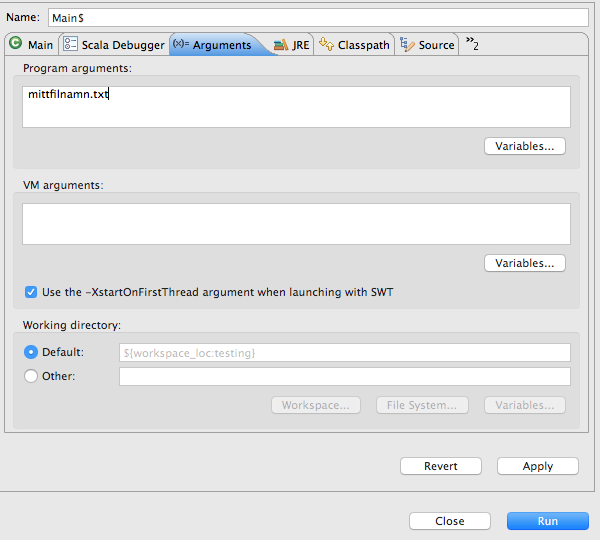
\includegraphics[width=0.5\textwidth]{../img/pirates/args.png} \\
\end{center}

Ändra i ditt program så att besättningen sparas till filen i det första argumentet om ett sådant har angivits, annars till filen \code{crew.txt}.

\Subtask Det går att överskugga toString() i \code{CrewMember} och på så sätt ändra utskriften genom att lägga till följande kodrad inne i klassen: 
\begin{Code}
override def toString(): String = ??? // add your code here. 
\end{Code}

\noindent Ändra utskriften så att den blir {\em snygg}, t ex med komma\\ 

\noindent Jack Sparrow, kapten \\
Anne Bonny, mordlysten matros \\
Ed Kenway, lönnmördare \\
... 
\newpage
\Task{Avlusa din besättning.}

\Subtask Din moraliska kompass hindrar dig inte från att också jobba för kungen. Hjälp honom att läsa listan!

En fil \code{fileName} kan läsas rad för rad till en vektor med följande kod som också finns i objektet \code{Utils}: 

\begin{Code}
// anropas t ex Utils.readLines("minFil.txt")
def readLines(fileName: String): Vector[String] = {
	   scala.io.Source.fromFile(fileName).getLines.toVector
	}
\end{Code}
Fyll i koden i \code{readCrew} som läser in besättningen från filen och skapar en \code{CrewMember} för varje rad. 

\Subtask Ändra i \code{main} för att testa att din besättning läses in från filen och skrivs ut dem i konsolen. Stämmer det med filinnehållet?

\Subtask Det går att följa exekveringen av programmet stegvis genom att köra det i \emph{debug mode} som startas med 

\includegraphics[width=0.05\textwidth]{../img/pirates/bug.png}

Då öppnas en debuggvy i Eclipse. Variablerna visas uppe i högra hörnet. Där går att klicka och se vilka värden varje variabel har för tillfället. 

Genom att lägga till \emph{break points} (klicka på sidan av koden för att lägga till och ta bort dem) kan programexekveringen pausas just innan raden exekveras  \\
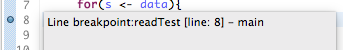
\includegraphics[width=0.5\textwidth]{../img/pirates/breakpoint.png} \\
så att programmeraren kan kontrollera variablernas värden och sen köra vidare med 
\includegraphics[width=0.05\textwidth]{../img/pirates/next.png}.

\Subtask Den konkurrerande kaptenen Charles Vane\footnote{hängd för sjöröveri i Port Royal 1721.} betalar dig för att sabotera listan genom att lägga till nonsensrader i filen. Gör det. Vad händer då när du exekverar ditt testprogram?

\Subtask Ändra din funktion \code{readCrew} så att en korrekt formaterad rad skapar en \code{CrewMember} medan felaktiga rader skriver ut felmeddelande.
Testa ditt nya program och se om det blir som förväntat genom lämpliga break points och utskrifter. Går det att lura ditt program?

\Task{Lögner, förbannade lögner och statistik.}\\
\noindent \\
För att du inte ska bli överlistad av dina sluga, lögnaktiga skeppskamrater behöver du kunna gissa hur en pirat tänker. Därför förkovrar du dig i Robert Louis Stevensons \emph{Skattkammarön}\footnote{Vars copyright har gått ut så du behöver inte piratkopiera den.} som finns i filen skattkammarön.txt i workspacet.  Genom att för varje ord spara det mest frekventa nästkommande ordet går det att förutse vad som kommer sägas\footnote{Detta används till exempel i Swiftkey på smarttelefoner.}. 

\Subtask Det går att läsa in ord från en fil med \code{scala.io.Source.fromFile} genom att först läsa in alla rader, ta bort allt som {\em inte} är svenska bokstäver och sen göra en split på \emph{white space}: 
\begin{CodeSmall}
// i Utils
def readWords(fileName: String): Vector[String] = {
	   scala.io.Source.fromFile(fileName).getLines.
	   map(_.replaceAll("[^a-zA-ZåäöÅÄÖ\\s]", " ")).
	   flatMap(_.split("\\s+")).filter(!_.isEmpty).toVector
	}
\end{CodeSmall}

Kodskelettet finns i objektet \code{PirateSpeech}. Lägg till kodrader i metoden \code{readBook} som läser in alla ord i filen skattkammarön.txt. Det finns en tom klass \code{FrequencyCounter} som för varje ord ska räkna nästkommande ord (sådana ordpar kallas bigram). Varje ord får en egen \code{FrequencyCounter} som i sin tur innehåller en samling, t ex en \code{Map} som listar alla efterföljande ord och deras antal så att vi kan få deras frekvens. Ditt uppdrag är att implementera \code{FrequencyCounter}.

\Subtask Lägg till en funktion \code{add(next:String)} i \code{FrequencyCounter} som ökar frekvensen av det ordet \code{next} eller lägger till det med räknaren satt till 1 om det inte finns. 

\Subtask Skriv ett program som läser in alla ord och räknar ut deras frekvens. Tips: håll reda på orden och deras bigramfrekvensräknare med en \\
\code{Map[String, FrequencyCounter]()}.

\Subtask Skriv funktionen \code{getBestGuess()} i \code{FrequencyCounter} som returnerar det mest frekventa efterföljande ordet. 

\Subtask Det tar lång tid att läsa hela boken varje gång programmet körs, det gäller att vara kvicktänkt och vi är faktiskt bara intresserade av den mest sannolika gissningen! Utöka din funktion \code{readBook} (eller skapa en ny funktion!) så att du sparar ordpar \code{word, bestGuess} med den bästa gissningen till varje ord till en fil. 

\Subtask Ändra i ditt program så att bara paren med de bästa gissningarna läses in i en \code{Map[String, String]()}. Fyll i metoden \code{testSpeech} som läser in ett ord från användaren från konsolen och gissar vad de ska säga sen. Efterföljs ''James'' oftast av ''Hawkins'' och eller av ''Flint''?


%\Task \emph{Read the map}. 

%\Subtask En underuppgift.

\subsection{Frivilliga extrauppgifter}

\Task Läs in större mängder text, implementera ett tangentbord till Android och bli rik.

%\Subtask En underuppgift.

%\Subtask En underuppgift.
    